\chapter{Progress of Mathematical Education in Thailand}

\begin{center}
{\em By}~ S. TANBUNYUEN
\end{center}
\medskip

\setcounter{pageoriginal}{150}
\textsc{When}\pageoriginale I first accepted our president's invitation to give you an account of what has been done in Thailand towards improving our mathematical training at the university and schools in the last four years, I felt that I had a chance of showing the progress that has been made along the lines planned at the last conference. But after compiling the facts and the events that happened, I am now not quite sure whether we are heading towards the right goad, or are even on the right path. So perhaps it might be a proper thing for me to say that this talk is about the changes in mathematical education in Thailand since 1956 and let you be the judge. There have certainly been many changes, change in the curriculum, in the text-books, and also in the quality of teachers, and if I may have your permission, I shall divide them into three parts, namely mathematics in schools, in training colleges, and in the university.

From the attached chart you will see that one must spend twelve years in school before one can go to the university. Of these twelve years, four are compulsory, and arithmetic is the only mathematics taught in these four grades. The time allotment varies from two to three hours per week for the first and second grades and from three to four hours per week for the third and fourth grades. Students are expected to be capable of doing all operations required in arithmetic and some simple mensurations.

The fifth grade marks the start of secondary education in Thailand, and for the next three years students are trained vigorously in arithmetic and practical geometry. Algebra is included when students reach the eighth grade, and at the eleventh grade trigonometry replaces arithmetic.

The content of the curriculum during the first ten years is still more or less the same as that in other countries. Generally, our 
\begin{figure}[H]
\centering
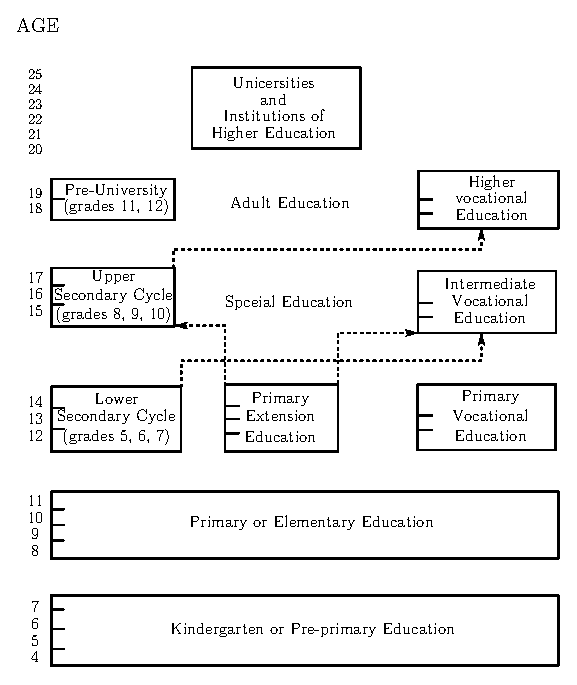
\includegraphics{figures/fig_02.eps}
\end{figure} 

\setcounter{pageoriginal}{152}
\noindent
students\pageoriginale have been known to be better calculators than other nationalities. This is because drills were imposed upon them, and mental arithmetic was given regularly in the class-room. With the increasing number of teachers trained in America came the new technique of teaching arithmetic. Teaching aids are now used extensively, instead of learning the multiplication table by rote. The Mathematical Society of Thailand is preparing new text-books for the ten grades. We hope we shall be able to publish the first four next May.

Lots of work has been done in using the project method of teaching from the fifth to the tenth grade. Students are encouraged to take active part in extra-curricular activities. Graphs and charts are introduced and used extensively by students in their study.

The mathematics taught during the last two years in school is still unsatisfactory. Even though students are divided into two groups. Arts and Science, the content is still below standard. Perhaps this is due to the fact that those responsible for the curriculum were trained in the U.S. and have not yet realised that American educationists are making great advances in this field. The new curriculum, which will go into effect next year, has combined algebra and statistics under the heading of general mathematics, with trigonometry and Euclidean geometry as separate subjects. General mathematics is compulsory for both arts and science students, while trigonometry and geometry are taught mainly to science students; trigonometry includes solution of triangles and functions of compound angles, multiple angles and quadrantal angles. The content of Euclidean geometry is now much reduced, and contains mainly the properties of triangles and circles with the stress on constructions.

Before students are allowed in Chulalongkorn University for science and engineering they have to pass an entrance examination, one of the papers being mathematics. This is a general mathematics paper which usually includes arithmetic, algebra, geometry and trigonometry. Since 1957 statistics has been included. The paper is prepared by me, and I always include a few problems which serve as an intelligence test.
\begin{figure}[H]
\centering
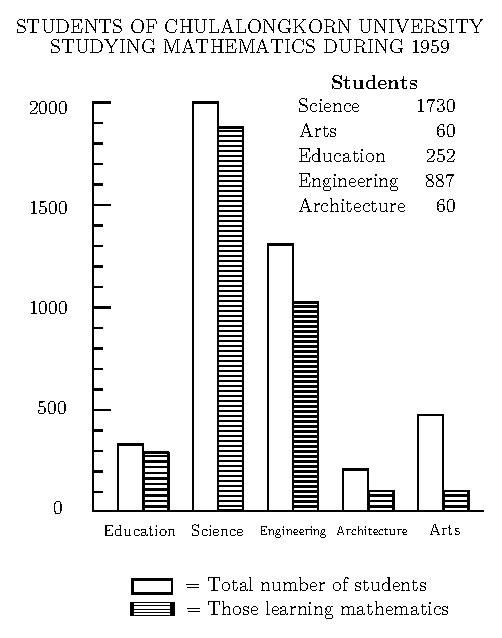
\includegraphics{figures/fig_03.eps}
\end{figure} 

\setcounter{pageoriginal}{154}
To\pageoriginale obtain a B.Sc. degree a student has to spend five years at the University and has to pass ten examinations, one every semester or half-year. Algebra and trigonometry are subjects taught in their first year. We used to give algebra during the first semester and trigonometry during the second semester. Since 1958 we have a combined course of algebra and trigonometry so that we can cut down outdated properties of polygons and circles in trigonometry and add the concept and nature of number to the course. Fortunately after spending a few days at the University of Chicago in 1957 I managed to obtain the lecture notes of College Mathematics for first year students, and adapted it for our students. In Thailand we divide our B.Sc. training into two parts.

The first part, which will take three years, is planned so that our students will be trained in all branches of science, namely mathematics, physics, chemistry and biology. They will be awarded a General Science Certificate at the end of three years and will be qualified as science teachers after another year of teacher training. Those students who are going into the medical profession later, will have to do at least two years of this course. To serve both the science and medical students two courses of mathematics are taught in the second year, namely calculus and analytic geometry, and statistics. We use the combined course of calculus and analytic geometry this year. Analytic geometry is taught from the vector concept and its content has been drastically cut to allow us to spend more time on the theoretical side of calculus. The result of the last semester is rather encouraging. My colleague, M. R. Pakpongsnit Snidwongs, is responsible for this course, and if any of you are interested in this experiment you can get information first hand from him.

You can see from our curriculum that we are not looking for able students in mathematics until the students enter their third year at the University. This is again rather unsatisfactory. I believe we are trying to give a sort of liberal arts education for the masses---there are 1564 science students in the first and second year.

When students reach their third year they are allowed to specialise and are required to choose only two subjects out of four. 
\begin{figure}[H]
\centering
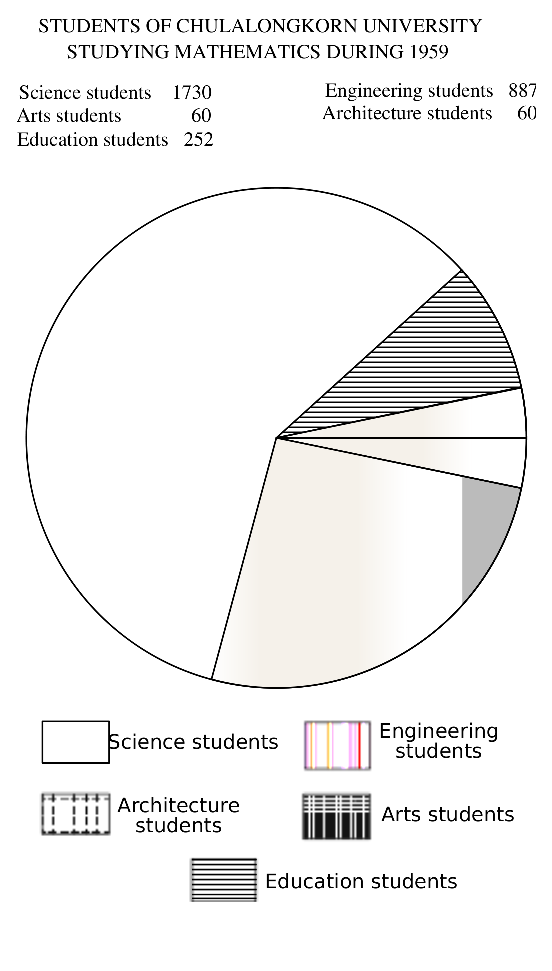
\includegraphics{figures/fig_04.eps}
\end{figure} 

\setcounter{pageoriginal}{156}
\indent
In\pageoriginale this year we continue with our calculus and analytic geometry, with introductions to differential equations and mechanics for those who want to spend more time on mathematics. It is our hope that some of them will go on with mathematics in their fourth and fifth years after taking their general science certificate.

This new curriculum of five years was started in June 1957. We shall know in June next year whether we shall have any student who specialises in mathematics.

The second part of the B.Sc. course in mathematics, which requires two years of study, is more or less the same as the last two years of the old syllabus. We have many elective courses but among the compulsory ones we have included modern algebra as an improvement. We were fortunate to have the services of an American mathematician for a year through the generosity of the United States Government and our staff have profited from his lecturing on modern algebra.

Not only do we teach mathematics to science and engineering students, we also serve the faculty of architecture and the faculties of arts and education. You can see from the charts that the number of students we teach is roughly three thousand a year. With 25 on the staff, only seven of whom have Master's degrees, you will agree with me that we are very much in need of qualified lecturers.

To improve the standard of mathematics teachers in schools, the Mathematical Society of Thailand has been giving summer courses to secondary school-teachers since 1956. When the Ministry of Education introduced statistics into the syllabus of high schools, we offered a course of statistics to teachers who otherwise are not able to teach it. For the last two summers we offered courses, with the approval of the Ministry of Education, to mathematics teachers. These courses are mainly algebra, geometry, and trigonometry, and include methods of teaching and teaching aids classes. About 600 teachers attend our courses, so that our mathematics teachers go back to their schools with more understanding of mathematics\pageoriginale in order to improve the mathematical instruction which is still badly neglected.

We discussed at our last conference the importance of good textbooks in mathematics. I am glad to report that the Mathematical Society of Thailand, through its monthly journal, has built up a good collection of mathematical articles in Thai. One of the contributors has written a text-book on probability which is being published in instalments in the journal. There have been many articles on the teaching of various subjects, as well as on the contents of the subjects themselves. The next issue of the journal will contain the notes on algebra taught at the University.

We have also taken on the job of writing text-books for schools, starting from the elementary, as reported earlier in this talk.

The Society has been promised support by the Teachers Association. The first four text-books for grade one to grade four will be published before June this year, and we hope we shall be able to publish the rest in due course. These text-books are written by committees, one for elementary, and others for lower secondary (grades 5, 6, 7), upper secondary (grades 8, 9, 10), and the pre-university (grades 11, 12).

There is still a lot of work to be done both by the Mathematical Society and the Department of Mathematics at Chulalongkorn University. So far we have not looked into the mathematics curriculum of the vocational schools and teachers' training colleges. Attempts are being made to increase the mathematics syllabus at the College of Education, where future teachers are trained under the guidance of Indiana University's Department of Education. To persuade educationists to recognise the importance of subject matter over the method of teaching requires a lot of patience and tact, of which I have very little indeed.

Text-books at the university level will be our next goal. So far the Department has been distributing notes from time to time to the first and second year students. There is a language difficulty at this level. The technical terms have to be done in English, while the\pageoriginale explanation is done in Thai. You will see from our journal specimens of this kind. Our student's knowledge of English is still inadequate, despite the fact that English is taught in all schools, and every student has taken a course in English for five years at least, before he comes to University. It will be some time before we can use English text-books in our first and second year.

Fortunately since 1958 we have acquired a library of modern mathematics text-books and journals through the generosity of the American Government and the Asia Foundation. It is now quite adequate for our needs and we hope to improve our stock annually from Government funds.

We are preparing the ground work for a graduate course in mathematics. The University is making plans for opening its graduate school next June with mathematics as one of the courses offered. Of research, there is very little to say. We have done experiments, with new texts and new approaches from the modern point of view but it is still too early to evaluate our efforts. The lack of experienced research mathematicians prevents us from working on original research, which has been our weak point since the establishment of the University 40 years ago.

\bigskip
\medskip
{\fontsize{9pt}{11pt}\selectfont
Chulalongkorn University

Thailand}\relax

